\addcontentsline{toc}{chapter}{Appendix}  % Add "Appendix" into the table of contents


\appendix

\chapter{Appendix}\label{app}

\section{Generalized SPA-NET application}\label{sec: generalized spa-net}
The SPA-NET architecture is based on the permutation symmetry of a physical process. This may allow people to extend the SPA-NET to a model which containing symmetry properties. In this appendix, two SM processes has been examined, all hadronic $t\bar{t}H$ decays ($t\bar{t}H$) and all hadronic four top decays ($t\bar{t}t\bar{t}$). The final state particles in these models contain permutation symmetry. This allows us to apply SPA-NET in these models. 
\subsection{All hadronic ttH decay process}\label{subsec: ttH}
The Figure \ref{fig:ttH} is the Feynmann diagram of all hadronic $t\bar{t}H$ decay ($t\bar{t}H$) processes. The final state particles of this process can be decomposed into three subsets, two particles from higgs boson, three particles from top quark, and three particles from anti-top quark. 
\\
In $t\bar{t}H$ process, there exists four b-jets and four quark jets. Same to the procedure for all hadronic top decay, we treat a jet as a b-jet by the b-tagging information from the detector simulation. Considering the b-tagging efficiency, the result provided in detector simulation will not always provide sufficient b-jets. A tighter cut(i.e.~require more b-jets/jets exists in an event) may rule out too many events due to the lack of b-jets. To avoid the problem of over-killing, the event selection for this model requires the event containing at least two b-jets and eight jets that passed the kinematics cuts.
\\
\begin{figure}[H]
	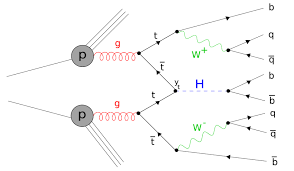
\includegraphics[width=0.7\linewidth]{Figures/all-had_ttH.png}
	\caption{Feynmann diagram of all hadronic ttH decay\cite{CMS:2019kgw}.}
	\label{fig:ttH}
\end{figure}
For the all hadronic ttH decay process, we apply the $\chi^{2}$ reconstruction (equation (\ref{eqn:chi2_ttH})) as the tradictional method.
\\
\begin{equation}\label{eqn:chi2_ttH}
	\chi^{2} = \frac{(m_{bqq'} - m_{\bar{b}q''q'''})^{2}}{\sigma^{2}_{\Delta_{\rm m_{bqq'}}}}  + \frac{(m_{qq'} - m_{\rm W})^{2}}{\sigma^{2}_{\rm W}} + \frac{(m _{q''q'''} - m_{\rm W})^{2}}{\sigma^{2}_{\rm W}} + \frac{(m_{b\bar{b}} - m_{\rm H})^{2}}{\sigma_{\rm H}^{2}}.
\end{equation} 
\subsection{All hadronic four top decay process}\label{subsec: four top}
The $t\bar{t}t\bar{t}$ is a process similar to the all hadronic top decay present in the main content but with more complicated final state particles. In this process, there exist twelve products and four subsets, each has one b-jet and 2 quark jets. This results in a four b-jets and eight quark jets final state with a higher computation complexity compare to $t\bar{t}$ process. The Figure \ref{fig:tttt} is the Feynmann diagram of $t\bar{t}t\bar{t}$ process. For the same reason mentioned in the second paragraph of Section \ref{subsec: ttH}, an event selection with two b-jets and twelve quark jets is implemented in this process. 
\\
\begin{figure}[H]
	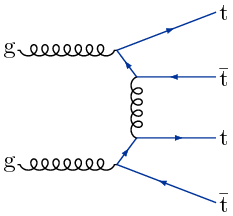
\includegraphics[width=0.5\linewidth]{Figures/four_top_LO.png}
	\caption{Feynmann diagram of all hadronic four top decay\cite{CMS:2017ocm}.}
	\label{fig:tttt}
\end{figure}
The definition of $\chi^{2}$ is similar to euqtion \ref{eqn:chi2} and has been generalized for all hadronic four top process.
\begin{equation}\label{eqn:chi2_tttt}
	\begin{split}
		\chi^{2} = &\frac{( m_{b_{1}q_{1}q_{2}} - m_{\rm t} )^{2}}{\sigma_{\rm t}^{2}} + \frac{( m_{\bar{b_{2}}q_{3}q_{4}} - m_{\rm t} )^{2}}{\sigma_{\rm t}^{2}} + \frac{(m_{q_{1}q_{2}} - m_{\rm W})^{2}}{\sigma^{2}_{\rm W}} + \frac{(m _{q_{3}q_{4}} - m_{\rm W})^{2}}{\sigma^{2}_{\rm W}} \\ 
		&\frac{( m_{b_{3}q_{5}q_{6}} - m_{\rm t} )^{2}}{\sigma_{\rm t}^{2}} + \frac{( m_{\bar{b_{4}}q_{7}q_{8}} - m_{\rm t} )^{2}}{\sigma_{\rm t}^{2}} + \frac{(m_{q_{5}q_{6}} - m_{\rm W})^{2}}{\sigma^{2}_{\rm W}} + \frac{(m _{q_{7}q_{8}} - m_{\rm W})^{2}}{\sigma^{2}_{\rm W}}.
	\end{split}	
\end{equation} 
\subsection{Reconstruct efficiency of generalized SPA-NET}\label{appendix_subsec: reco eff}
Since the computation of $\chi^{2}$ method for the $t\bar{t}t\bar{t}$ and $t\bar{t}H$ process is too complicated (i.e.~needs a lots of time), the comparison between $\chi^{2}$ method and SPA-NET is not shown in this appendix. After the computation, the $\chi^{2}$ method provides a very low reconstruct efficiency. Considering 100 events, the $\chi^{2}$ method needs more than one day and the reconstruct efficiency is less than 10\% (using Python). The reconstruct efficiency of SPA-NET applies to ttH process is shown in Table \ref{tab:tth_spanet_2btag}.
\\
For comparison, we separate the dataset into several cases which contain reconstructable higgs boson, and the event with one or two reconstructable top quarks. Furthermore, we decompose these cases by the number of jets exist in an event. The  \textbf{event efficiency} and  \textbf{Higgs/Top quark efficiency} using the same definition in \ref{tab:eps}.  The \textbf{Event Fraction} is the percentage of total events included in the denominator for the efficiency calculations.
\\
The result shown in the Table \ref{tab:tth_spanet_2btag} and Table \ref{tab:tttt_spanet_2btag} provides evidence for the application of SPA-NET. In the $t\bar{t}H$ process, the SPA-NET can reconstruct with an event efficiency around 30\% in our validation dataset. SPA-NET has the peak of performance when considering the event which has three reconstructable particles with an efficiency 31.7\%. In the per-quark level, the SPA-NET can reconstruct either higgs boson and top quark with at least 40\% efficiency. 
\\
\begin{table}[H]
	\resizebox{13cm}{!}{
		\begin{tabular}{c | c | c | c c c}
\hline
\hline
& $N_\mathrm{jets}$ & Event Fraction & Event Efficiency & Higgs Efficiency & Top Quark 
Efficiency\\
\hline
All Events&== 8 & 0.281 & 0.329 & 0.430 & 0.498\\
&== 9 & 0.316 & 0.304 & 0.430 & 0.476\\
&$\geq 10$ & 0.355 & 0.264 & 0.420 & 0.441\\
&\textbf{Inclusive} & \textbf{0.954} & \textbf{0.297} & \textbf{0.426} & \textbf{0.468}\\
\hline
\hline
Higgs Events&== 8 & 0.197 & 0.317 & 0.430 & 0.531\\
&== 9 & 0.227 & 0.295 & 0.430 & 0.504\\
&$\geq 10$ & 0.261 & 0.257 & 0.420 & 0.462\\
&\textbf{Inclusive} & \textbf{0.686} & \textbf{0.287} & \textbf{0.426} & \textbf{0.493}\\
\hline
\hline
1 Top Events&== 8 & 0.167 & 0.314 & 0.413 & 0.466\\
&== 9 & 0.177 & 0.297 & 0.409 & 0.448\\
&$\geq 10$ & 0.184 & 0.273 & 0.397 & 0.421\\
&\textbf{Inclusive} & \textbf{0.529} & \textbf{0.294} & \textbf{0.406} & \textbf{0.444}\\
\hline
\hline
2 Top Events&== 8 & 0.066 & 0.352 & 0.590 & 0.539\\
&== 9 & 0.092 & 0.295 & 0.540 & 0.504\\
&$\geq 10$ & 0.130 & 0.225 & 0.490 & 0.456\\
&\textbf{Inclusive} & \textbf{0.289} & \textbf{0.277} & \textbf{0.526} & \textbf{0.490}\\
\hline
\hline
Full Events&== 8 & 0.036 & 0.440 & 0.590 & 0.599\\
&== 9 & 0.057 & 0.344 & 0.540 & 0.542\\
&$\geq 10$ & 0.087 & 0.248 & 0.490 & 0.480\\
&\textbf{Inclusive} & \textbf{0.180} & \textbf{0.317} & \textbf{0.526} & \textbf{0.523}\\
\hline
\hline
\end{tabular}
    
	}
	\vspace{0.1cm}
	\caption{SPA-NET results on all hadronic ttH decay with at least $two$ b-tagged jets (all generated events). The ``all events'' category is the whole dataset without selections. The ``higgs events'' is a case considering the event that contains a reconstructable higgs boson. Top events focus on the category that has one or two reconstructable top quarks. Full events mean the events in this category should include all reconstructable targets.}
	\label{tab:tth_spanet_2btag}
\end{table}
For $t\bar{t}t\bar{t}$ process which is the most complicated case, the SPA-NET still provides an event efficiency around 40\% in one top event. The low event efficiency appears in the full event and the case with two or more reconstructable top quarks is expected. These cases are much more complicated than other cases and cannot be improved by the partial event training which feeds the in-complete input data to the network.  
\begin{table}[H]
	\resizebox{12cm}{!}{
		\begin{tabular}{c | c | c | c c c}
\hline
\hline
& $N_\mathrm{jets}$ & Event Fraction & Event Efficiency &Top Quark Efficiency\\
\hline
All Events&== 12 & 0.227 & 0.257 & 0.458\\
&== 13 & 0.309 & 0.232 & 0.453\\
&$\geq 14$ & 0.433 & 0.185 & 0.426\\
&\textbf{Inclusive} & \textbf{0.970} & \textbf{0.217} & \textbf{0.441}\\
\hline
\hline
1 Top Events&== 12 & 0.060 & 0.412 & 0.412\\
&== 13 & 0.069 & 0.399 & 0.399\\
&$\geq 14$ & 0.073 & 0.374 & 0.374\\
&\textbf{Inclusive} & \textbf{0.202} & \textbf{0.394} & \textbf{0.394}\\
\hline
\hline
2 Top Events&== 12 & 0.106 & 0.217 & 0.441\\
&== 13 & 0.136 & 0.206 & 0.430\\
&$\geq 14$ & 0.172 & 0.181 & 0.406\\
&\textbf{Inclusive} & \textbf{0.415} & \textbf{0.198} & \textbf{0.423}\\
\hline
\hline
3 Top Events&== 12 & 0.056 & 0.162 & 0.482\\
&== 13 & 0.089 & 0.148 & 0.471\\
&$\geq 14$ & 0.148 & 0.117 & 0.436\\
&\textbf{Inclusive} & \textbf{0.294} & \textbf{0.135} & \textbf{0.455}\\
\hline
\hline
4 Top Events&== 12 & 0.005 & 0.297 & 0.580\\
&== 13 & 0.014 & 0.211 & 0.543\\
&$\geq 14$ & 0.039 & 0.111 & 0.470\\
&\textbf{Inclusive} & \textbf{0.059} & \textbf{0.152} & \textbf{0.497}\\
\hline
\hline
\end{tabular}

    
	}
	\vspace{0.1cm}
	\caption{SPA-NET results on all hadronic tttt decay with at least $2$ btagged jets (all generated events).}
	\label{tab:tttt_spanet_2btag}
\end{table}
In summary, SPA-NET can be applied to the physical process which satisfies permutation symmetry with an acceptable result. There is still a large room for improvement in such a complicated process, but the ability for generalizing SPA-NET has been prooved.
\newpage
\section{Reduction of computating time}\label{sec: reduction CPU time}
\begin{figure}[H]
	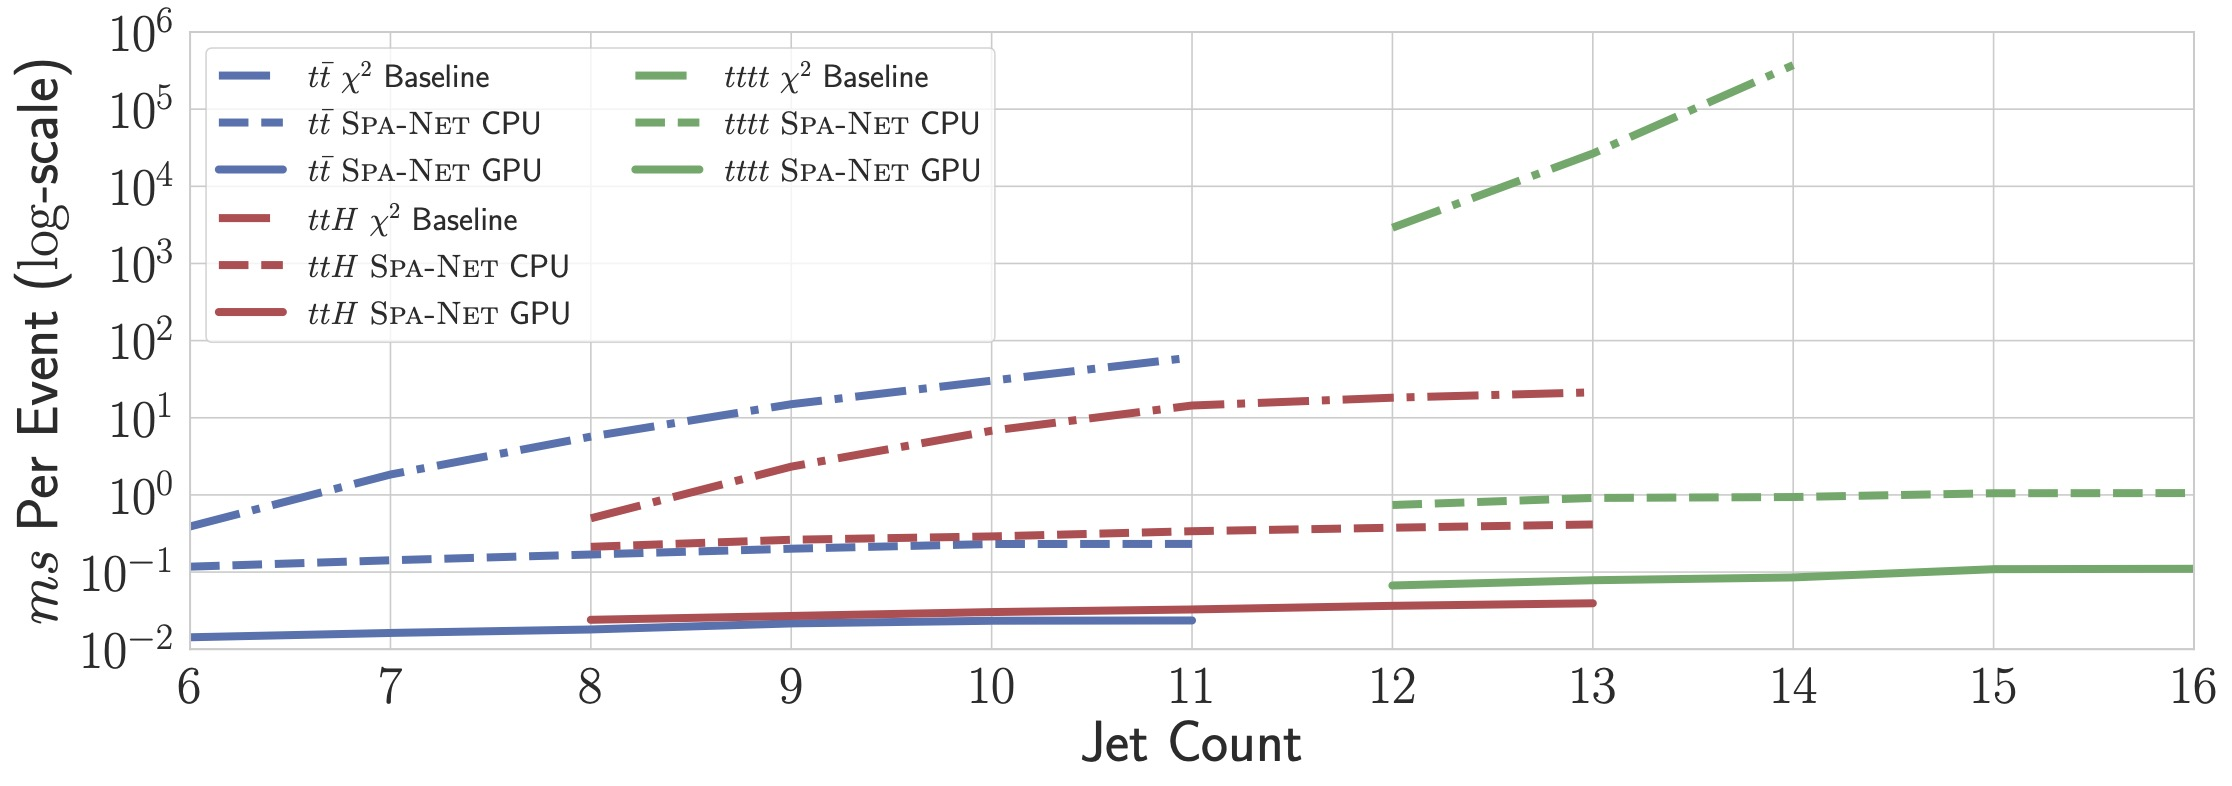
\includegraphics[width=1.0\linewidth]{Figures/timing_plot.jpg}
	\caption{ Average run-time for jet-assignment inference of SPA-NET and χ
		2 on various events
		and jet multiplicities over 1000 runs. SPA-NETs were evaluated with a batch size of 1024 events.
		Timings are performed on an Intel I7 10700K CPU with 64 GB of RAM and Nvidia 3080 GPU.}
	\label{fig:timing}
\end{figure}
The SPA-NET has a lower computational complexity thanks to the architecture that no need to iterate all the possible combinations. The Figure \ref{fig:timing} provided a comarison of average run-time for $\chi^{2}$ and SPA-NET in $t\bar{t}$, $t\bar{t}H$, and $t\bar{t}t\bar{t}$ process. We can see SPA-NET provide a better run-time performance in call categories.  
\pagebreak 